% ------------------------------------------------------------------------------
% TYPO3 Version 9.1 - What's New - Chapter "Introduction" (Serbian Version)
%
% @author	Michael Schams <schams.net>
% @license	Creative Commons BY-NC-SA 3.0
% @link		http://typo3.org/download/release-notes/whats-new/
% @language	English
% ------------------------------------------------------------------------------
% LTXE-CHAPTER-UID:		7fdf26cc-362160ab-d6c8b905-19722b20
% LTXE-CHAPTER-NAME:	Introduction
% ------------------------------------------------------------------------------

\section{Uvod}
\begin{frame}[fragile]
	\frametitle{Uvod}

	\begin{center}\huge{Uvod}\end{center}
	\begin{center}\huge{\color{typo3darkgrey}\textbf{Cinjenice}}\end{center}

\end{frame}

% ------------------------------------------------------------------------------
% LTXE-SLIDE-START
% LTXE-SLIDE-UID:		6aae5c47-13009e8e-c2cf644d-5054ebc6
% LTXE-SLIDE-ORIGIN:	db9ce9bf-51fe8c3b-c6a2649f-aa7018b5 English
% LTXE-SLIDE-TITLE:		TYPO3 Version 9.1 - The Facts
% ------------------------------------------------------------------------------
\begin{frame}[fragile]
	\frametitle{Uvod}
	\framesubtitle{TYPO3 Verzija 9.1 - Cinjenice}

	\begin{itemize}
		\item Datum objavljivanja: 30 Januar 2018
		\item Tip objavljivanja: Brza objava (Sprint Release)
	\end{itemize}

	\begin{figure}
		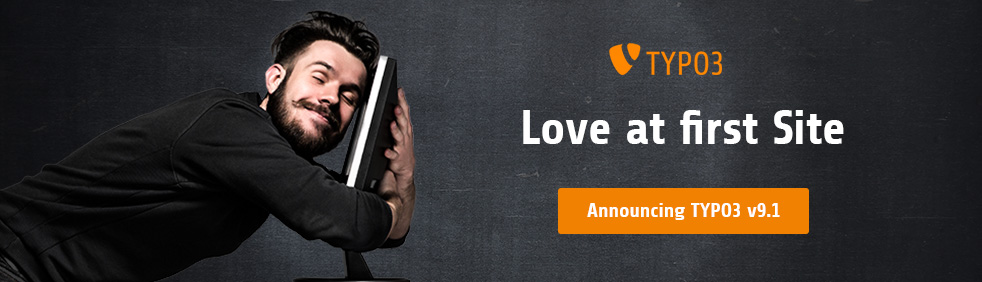
\includegraphics[width=0.95\linewidth]{Introduction/typo3-v91-banner.jpg}
	\end{figure}

\end{frame}

% ------------------------------------------------------------------------------
% LTXE-SLIDE-START
% LTXE-SLIDE-UID:		686ea9b7-1d7455b7-7b7454b9-8edab6ba
% LTXE-SLIDE-ORIGIN:	baf0e8fa-b8335fbe-911020ab-489d6156 English
% LTXE-SLIDE-TITLE:		System Requirements
% ------------------------------------------------------------------------------
\begin{frame}[fragile]
	\frametitle{Uvod}
	\framesubtitle{Sistemski zahtevi}

	\begin{itemize}
		\item PHP verzija 7.2\newline
			\smaller
				(verovatno ce se ovaj zahtev spustiti na PHP 7.1 ili 7.0 za naredne objave, odluka jos nije donesena)
			\normalsize

		\item PHP podesavanja:

			\begin{itemize}
				\item \texttt{memory\_limit} >= 128M
				\item \texttt{max\_execution\_time} >= 240s
				\item \texttt{max\_input\_vars} >= 1500
				\item opcija \texttt{-}\texttt{-disable-ipv6} \underline{ne sme} se koristit
			\end{itemize}

		\item Vecina DB servera koji rade sa \textbf{Doctrine DBAL} rade takodje i sa TYPO3.
			Testirani DB serveri su:
	\end{itemize}

	\begin{figure}
		
\includegraphics[width=0.70\linewidth]{Introduction/logo-databases.png}
	\end{figure}

\end{frame}

% ------------------------------------------------------------------------------
% LTXE-SLIDE-START
% LTXE-SLIDE-UID:		b67b6cba-5558a164-7d63726b-0d61d23c
% LTXE-SLIDE-ORIGIN:	dfe5c3a8-72a55162-da879770-778ebfec English
% LTXE-SLIDE-TITLE:		Development, Release and Maintenance Timeline
% ------------------------------------------------------------------------------
\begin{frame}[fragile]
	\frametitle{Uvod}
	\framesubtitle{Razvoj, objavljivanje i vreme odrzavanja}

	\textbf{TYPO3 v9}

	\begin{figure}
		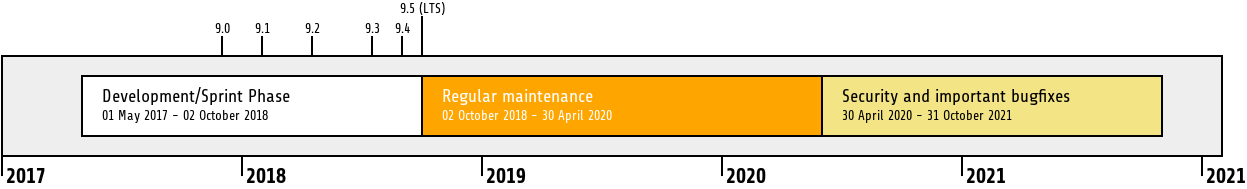
\includegraphics[width=1\linewidth]{Introduction/typo3-v9-lifecycle.png}
	\end{figure}

	\textbf{Produzeno vreme podrske}\newline
	\smaller
		\href{https://typo3.com}{TYPO3 GmbH} nudi dodatne opcije za podrsku za TYPO3 v9 LTS 
		cak i posle 31. Oktobra 2021 za dodatne dve godine.
	\normalsize

%	\url{https://typo3.com/our-services/extended-support/}

\end{frame}

% ------------------------------------------------------------------------------
% LTXE-SLIDE-START
% LTXE-SLIDE-UID:		8d3bf494-9e353764-99470b7b-c78415e5
% LTXE-SLIDE-ORIGIN:	1c2b096f-e4e0a65c-b0b0d84b-e18889a1 English
% LTXE-SLIDE-TITLE:		TYPO3 v9 Roadmap
% ------------------------------------------------------------------------------
\begin{frame}[fragile]
	\frametitle{Uvod}
	\framesubtitle{TYPO3 v9 plan}

	Predvidjeni datumi objavljivanja i njihov osnovni fokus:

	\begin{itemize}

		\item v9.0 \tabto{1.1cm}12/Dec/2017\tabto{3.4cm}Install Tool i Page Tree Refactoring,\newline
			\tabto{3.4cm}Ujedinjen prevod strana
		\item
			\begingroup
				\color{typo3orange}
					v9.1 \tabto{1.1cm}30/Jan/2018\tabto{3.4cm}Upravljanje redirekcijama
			\endgroup
		\item v9.2 \tabto{1.1cm}10/Apr/2018\tabto{3.4cm}Konfiguracija sajta
		\item v9.3 \tabto{1.1cm}12/Jun/2018\tabto{3.4cm}URL rutiranje
		\item v9.4 \tabto{1.1cm}04/Sep/2018\tabto{3.4cm}Uredjivanje Frontend-a
		\item v9.5 \tabto{1.1cm}02/Oct/2018\tabto{3.4cm}LTS objava

	\end{itemize}

	\smaller
		\url{https://typo3.org/news/article/typo3-v9-roadmap/}
	\normalsize

\end{frame}

% ------------------------------------------------------------------------------
% LTXE-SLIDE-START
% LTXE-SLIDE-UID:		b74ffb1e-c0f98cc1-0ee6bbca-9b6857e2
% LTXE-SLIDE-ORIGIN:	27b13d1c-5c952e3e-d4422d93-0a8a273d English
% LTXE-SLIDE-TITLE:		Installation
% ------------------------------------------------------------------------------
\begin{frame}[fragile]
	\frametitle{Uvod}
	\framesubtitle{Instalacija}

	\begin{itemize}
		\item Zvanicna \textit{klasicna} procedura za instalaciju na Linux/Mac OS\newline
			(DocumentRoot na primer \texttt{/var/www/site/htdocs}):
		\begin{lstlisting}
			$ cd /var/www/site
			$ wget --content-disposition get.typo3.org/9.1
			$ tar xzf typo3_src-9.1.0.tar.gz
			$ cd htdocs
			$ ln -s ../typo3_src-9.1.0 typo3_src
			$ ln -s typo3_src/index.php
			$ ln -s typo3_src/typo3
			$ touch FIRST_INSTALL
		\end{lstlisting}

		\item Simbolicki linkovi (Symbolic links) na Microsoft Windows:

			\begin{itemize}
				\item Koristiti \texttt{junction} za Windows XP/2000
				\item Koristiti \texttt{mklink} za Windows Vista i Windows 7 i novije
			\end{itemize}

	\end{itemize}
\end{frame}

% ------------------------------------------------------------------------------
% LTXE-SLIDE-START
% LTXE-SLIDE-UID:		0f59de4f-1c8e5cd1-dd007b99-0e73f060
% LTXE-SLIDE-ORIGIN:	2991c08b-8831f59c-56bc188c-e05b8e92 English
% LTXE-SLIDE-TITLE:		Installation using composer
% ------------------------------------------------------------------------------
\begin{frame}[fragile]
	\frametitle{Instalacija i nadogradnja}
	\framesubtitle{Instalacija koriscenjem \texttt{composer}}

	\begin{itemize}
		\item Instalacija koriscenjem \textit{composer} na Linux/Mac OS X

			\begin{lstlisting}
				$ cd /var/www/site/
				$ composer create-project typo3/minimal
			\end{lstlisting}

		\item Alternativno, napravite Vas \texttt{composer.json} fajl i pokrenite:

			\begin{lstlisting}
				$ composer install
			\end{lstlisting}

			Primer \texttt{composer.json} fajla mozete skinuti sa:\newline
			\small
				\href{https://git.typo3.org/TYPO3CMS/Distributions/Base.git/blob/HEAD:/composer.json}{git.typo3.org/TYPO3CMS/Distributions/Base.git/blob/HEAD:/composer.json}
			\normalsize

	\end{itemize}
\end{frame}

% ------------------------------------------------------------------------------
% LTXE-SLIDE-START
% LTXE-SLIDE-UID:		88df68ba-b9dbc2c6-f11a708d-f9a650b0
% LTXE-SLIDE-ORIGIN:	3bc1e21e-cf2c23c4-b1d641af-8e351b92 English
% LTXE-SLIDE-TITLE:		Upgrade to TYPO3 Version 9
% ------------------------------------------------------------------------------
%\begin{frame}[fragile]
%	\frametitle{Uvod}
%	\framesubtitle{Nadogradnja na TYPO3 varziju 9.x}
%
%	\begin{itemize}
%		\item Nadogradnja je moguca samo sa TYPO3 v8 LTS
%		\item TYPO3 < v8 LTS bi prvo trebalo nadograditi na TYPO3 v8 LTS
%	\end{itemize}
%
%	\begin{itemize}
%
%		\item Upsutstvo za nadogradnju:\newline
%			\smaller\url{https://wiki.typo3.org/Upgrade#Upgrading_to_9.1}\normalsize
%		\item Zvanicni TYPO3 vodic "TYPO3 Installation and Upgrading":
%			\smaller\url{https://docs.typo3.org/typo3cms/InstallationGuide}\normalsize
%		\item Opsti pristup:
%			\begin{itemize}
%				\item Proveriti minimalne sistemske zahte \small(PHP, MySQL, itd.)
%				\item Proveriti \textbf{deprecation\_*.log} u staroj TYPO3 instanci
%				\item Nadograditi sva prosirenja na najnoviju verziju
%				\item Postaviti nove fajlove i pokrenuti Install Tool -> Upgrade Wizard
%				\item Proveriti startup modul za administratore (opciono)
%			\end{itemize}
%	\end{itemize}
%
%\end{frame}
%
% ------------------------------------------------------------------------------
